\newpage

\section{Dynamic Code Optimization}

Most materials are based on \cite{whaley2001partial} in this section.

Dynamic compilation systems explore an interesting tradeoff. On one hand, we would like to have code performance
that is comparable to static compilation techniques. However, we would also like to avoid long startup delays, long
latencies, and slow responsiveness, which implies that the
dynamic compiler should be fast.

Many dynamic compilation systems attack this problem by
using an interpreter and an optimizing compiler. They begin
by interpreting the code, and when the execution count for
the method reaches a certain threshold or by some other
heuristic, they use the optimizing compiler to dynamically
compile the code for the method\cite{suganuma2000overview,paleczny2001java} . Some systems
use a fast code generator (baseline compiler) rather than an
interpreter \cite{burke1999jalapeno, cierniak2000practicing}.

The problem with these systems is that the execution speed
of the interpreted or baseline compiled code is significantly
worse than that of fully optimized code — typically 30\% to
ten times slower for baseline compiled code \cite{burke1999jalapeno, cierniak2000practicing} and ten
to a hundred times slower for interpreted code \cite{suganuma2000overview,paleczny2001java}.
Therefore, we would like to transfer into the optimized version as quickly as possible. However, the optimizing compiler can take a long time to compile. Waiting for the optimizing compiler to finish hurts program startup and response times. Some systems use a multi-level compilation
approach, whereby they progress through a number of different compilation “levels”, and thereby slowly “accelerate”
into optimized execution \cite{paleczny2001java,suganuma2001dynamic}. However, this simply
exacerbates the problem of having a long delay until the
program runs at full speed.

Unlike interpretation, compilation takes time that is proportional to the amount of code that is being compiled. Many
analyses and optimizations are superlinear in the size of the
code (basic blocks, instructions, registers, etc.) This can
cause the compilation time to increase significantly as the
amount of code being compiled gets large. Compilation of
large amounts of code is the cause of undesirably long compilation times.


However, when compiling a method at a time, we do not
really have much choice in the matter. Some methods are
large to begin with, and others grow large after performing
inlining. Even when being frugal and inlining only when it
will make a noticeable difference in performance, methods
can still grow large, and excessively restricting inlining can
significantly hurt performance \cite{suganuma2000overview}.


The root of the problem is that method boundaries do not
correspond to the code that would most benefit from optimizing compilation. Even “hot” methods typically contain
some code that is rarely or never executed, but often contain frequently-executed call sites to methods (which in turn,
contain their own rarely-executed code.) Figure \ref{fig:p174} contains a
paraphrased example from the spec db benchmark. In
this example, the \texttt{readdb} method is hot due to the while
loop that it contains. However, the error handling code
guarded by the if and the exception handler are rarely
executed. Likewise, the call to \texttt{read()} is in the loop and
therefore a good candidate for inlining. However, \texttt{read()}
itself contains rarely-executed error handling code. The region that is important to compile — the while loop and the
hot path in \texttt{read()} — have nothing to do with the method
boundaries. Using a method granularity causes the compiler
to waste time compiling and optimizing large pieces of code
that do not matter.


\begin{figure}[H]
	\centering
	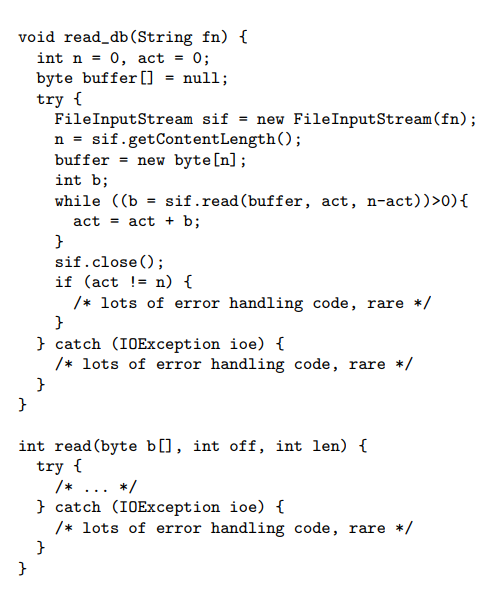
\includegraphics[width=0.5\textwidth]{p174.png}
	\caption{From spec db. Method boundaries do not
    correspond well to where the time is actually spent.}
	\label{fig:p174}
\end{figure}

John Whaley\cite{whaley2001partial} describes a technique to selectively compile and
optimize partial methods. This gives us much better control
over what we spend time compiling and optimizing. This
technique uses dynamic profile data to make a prediction of
what code will actually be executed, and selectively compiles and optimizes only that code. If the program actually
attempts to branch to code that was not compiled (so-called
“rare code”), the system falls back to interpretation or another dynamically compiled version.

\subsection{Partial Method Compilation}


view
The general idea of the technique is to replace all entries
into rare blocks with stubs that transfer control to the interpreter. The rare blocks are completely removed from the
compiler’s intermediate representation. Only very minimal
changes to the compiler are necessary; optimizations can
optionally use rare block information to attempt to better
optimize the common paths. At the end of compilation, we
store a map corresponding to each interpreter transfer point,
which specifies how to reconstruct the interpreter state at
that point.


We now describe each step of the process in detail.


\textbf{1. Based on profile data, determine the set of rare
blocks.}
The entry points of the rare basic blocks
are mapped to abstract program locations, which then used to mark basic blocks as rare in the compiler’s
intermediate representation.

\textbf{2. Perform live variable analysis.}
Before any transformations are performed, we perform
live variable analysis to determine the set of live variables at rare block entry points.

\begin{figure}[H]
	\centering
	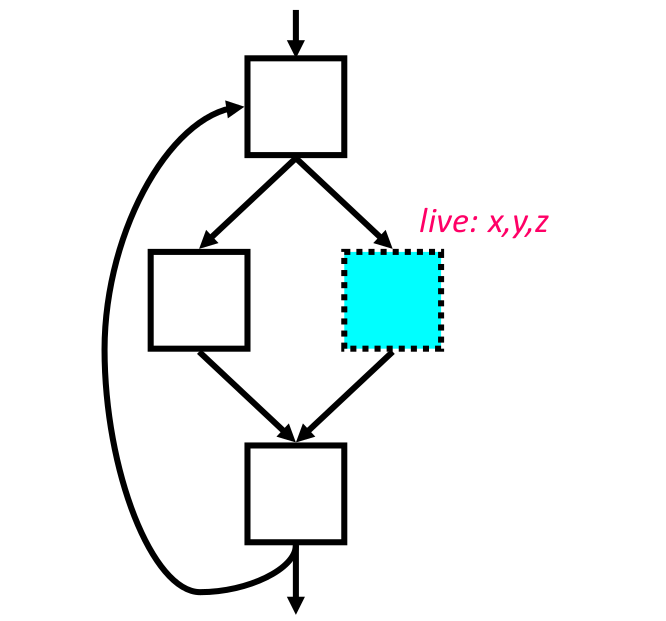
\includegraphics[width=0.3\textwidth]{p176.png}
	\caption{Determine the set of live variables at rare block entry points.}
	\label{fig:p176}
\end{figure}

\textbf{3. Redirect the control flow edges that targeted
rare blocks, and remove the rare blocks.}
For each control flow edge from a non-rare block to a
rare block, we generate a new basic block containing
a single instruction that transfers control to the interpreter. This instruction uses all local variables and
Java stack locations from the Java bytecode that are
live at that point. We redirect the control flow edge
to point to this new block, and add an edge from the
new block to the exit node. See Figure \ref{fig:p177} for an example. After this process, rare blocks can be removed
as unreachable code.


\begin{figure}[H]
	\centering
	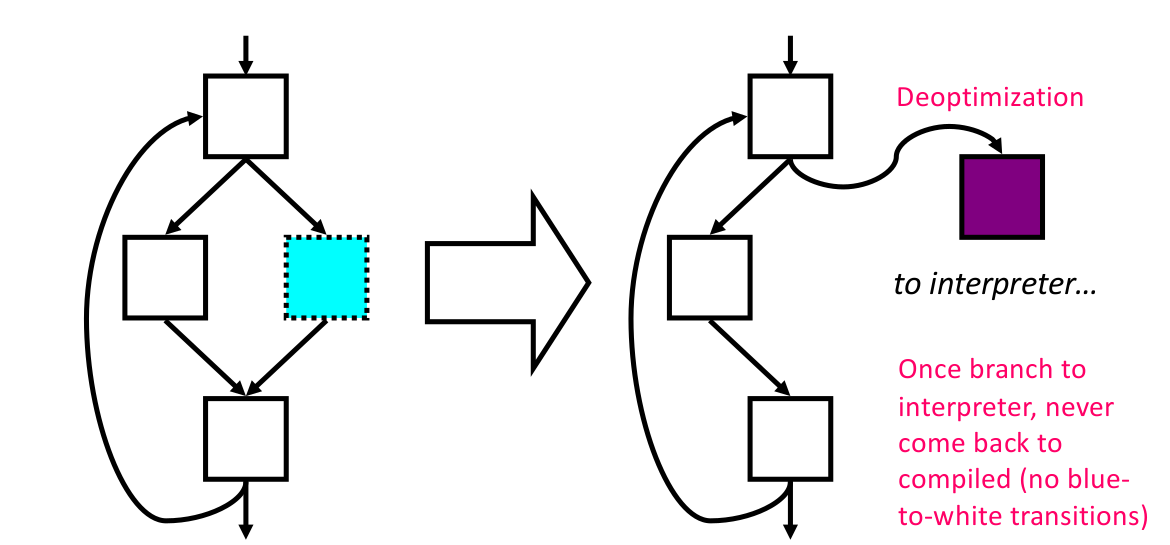
\includegraphics[width=0.5\textwidth]{p177.png}
	\caption{An example of redirecting the rare path.
    On the left, the dotted block is rare, so we redirect
    it to a block that calls the interpreter.}
	\label{fig:p177}
\end{figure}

\textbf{4. Perform compilation normally.}
All analysis, optimization, and code generation proceeds normally. Analyses treat the interpreter transfer
point as an unanalyzable method call. 

\begin{figure}[H]
	\centering
	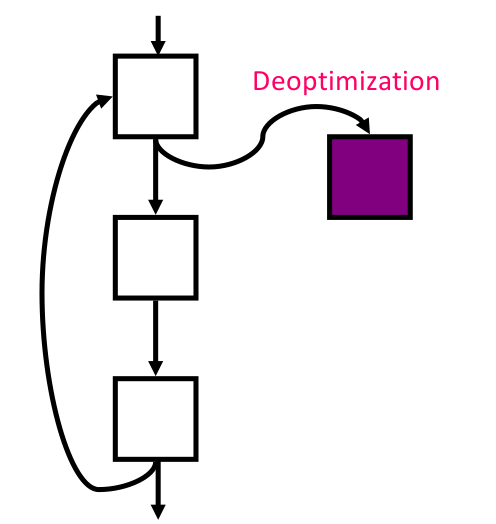
\includegraphics[width=0.3\textwidth]{p178.png}
	\caption{Analyses treat the interpreter transfer point as an unanalyzable method call.}
	\label{fig:p178}
\end{figure}

\textbf{5. Record a map for each interpreter transfer
point.}
When generating the code to call the glue routine, we
also generate a map that specifies the location, in registers or memory, of each of the local variables and
Java stack locations used in the original Java bytecode.
This map is used by the glue routine to reconstruct the
interpreter state. The map is stored immediately after the call in the instruction stream. Each map is
typically under 100 bytes long.


\begin{figure}[H]
	\centering
	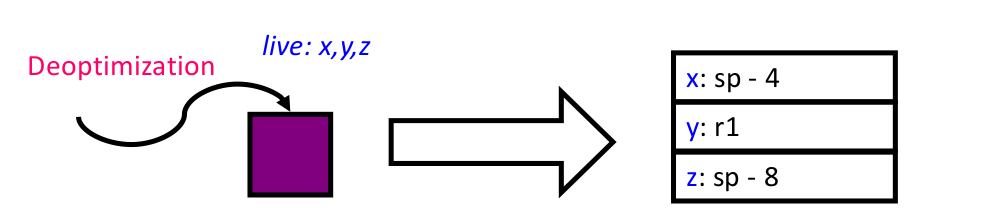
\includegraphics[width=0.5\textwidth]{p179.png}
	\caption{In code generation, generate a map that specifies the location, in registers
    or memory, of each of the live variables used to reconstruct the interpreter state}
	\label{fig:p179}
\end{figure}




\subsection{Partial dead code elimination}

We modified our dead code elimination algorithm to treat
rare blocks specially. This allows us to move computation
that is only live on a rare path into the rare block, saving
computation in the common case.
Our dead code elimination uses an optimistic approach similar to the one described by Muchnick \cite{muchnick1997advanced}, originally due to
Kennedy \cite{kennedy1979survey}. That analysis begins by marking all instructions that compute essential values, and then recursively marking all instructions that contribute to the computation
of essential values. Any non-essential instructions are then
eliminated.

Our analysis operates on SSA form. It first computes the
essential instructions in all non-rare blocks, completely ignoring all rare blocks. An essential instruction computes a
value that is used in a predicate, returned or output by the
method, or has a potential side-effect.
It then visits each
rare block to discover instructions that are essential for that
rare block, but not essential for non-rare blocks. If these
instructions are recomputable at the point of the rare block,
they can be safely copied there.


For each instruction in the rare block, it recursively visits
all instructions that contribute to the computation of values
for that instruction. If an instruction is marked as essential,
it is skipped. If it is a $\Phi$ function, it depends on an earlier
predicate, and is therefore (recursively) marked as essential.
Otherwise, the instruction is added to a set of instructions
associated with the rare block.
After computing sets for all rare blocks, it adds each of the
non-essential instructions in a set to its corresponding rare
block. Then, all instructions in non-rare blocks that are not
marked as essential are eliminated.


Now we make an argument of correctness. Any instruction
that was eliminated on the main path either computed a
value that was not essential anywhere, in which case it is
obviously correct to eliminate it, or it was only essential in
some number of rare blocks, in which case it would have
been copied into those rare blocks. Copying the instruction
into a rare block is legal because, as the instruction is not a $\Phi$
function, the instruction dominates and is in the same loop
as the rare block and therefore would have executed exactly
once. Also, any instruction with a potential side effect or
that read from or wrote to memory would have been marked
as essential on the main path and therefore executed in its
original location. Therefore, moving the instruction to a
rare block does not violate exception or memory semantics.

\begin{figure}[H]
	\centering
	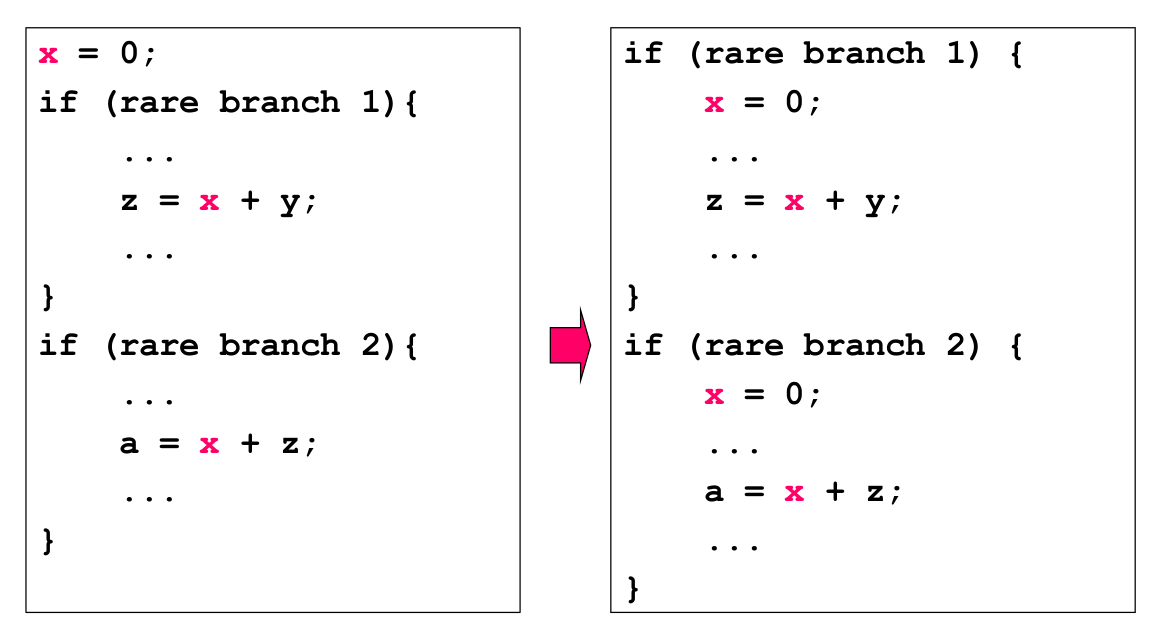
\includegraphics[width=0.6\textwidth]{p180.png}
	\caption{Partial Dead Code Example.}
	\label{fig:p180}
\end{figure}